
\documentclass{article} % For LaTeX2e
\usepackage{iclr2025_conference,times}

% Optional math commands from https://github.com/goodfeli/dlbook_notation.

\theoremstyle{plain}
\newtheorem{theorem}{Theorem}
\newtheorem{lemma}{Lemma}[section]
\newtheorem{proposition}[lemma]{Proposition}
\newtheorem{corollary}[lemma]{Corollary}
\theoremstyle{definition}
\newtheorem{definition}[lemma]{Definition}
\newtheorem{assumption}[lemma]{Assumption}
\theoremstyle{remark}
\newtheorem{remark}[lemma]{Remark}


\newcommand{\diag}{\mathrm{diag}}
\newcommand{\norm}[1]{\left\|{#1}\right\|} %
\newcommand{\rank}{\mathrm{rank}}
\newcommand{\B}{\mathcal{B}}
\newcommand{\M}{\mathcal{M}}
\newcommand{\BS}{\B^*}
\newcommand{\BBS}{\B\B^*}
\newcommand{\BSB}{\B^*\B}
\newcommand{\MMS}{\M\M^*}
\newcommand{\MSM}{\M^*\M}
\newcommand{\BF}{\mathcal{B}\mathcal{F}}
\newcommand{\BD}{\mathcal{B}\mathcal{D}}
\newcommand{\DB}{\mathcal{D}\mathcal{B}}
\newcommand{\ind}[1]{^{(#1)}}

\newcommand{\vzero}{\mathbf{0}}
\newcommand{\vone}{\mathbf{1}}
\newcommand{\va}{\mathbf{a}}
\newcommand{\vb}{\mathbf{b}}
\newcommand{\vc}{\mathbf{c}}
\newcommand{\vd}{\mathbf{d}}
\newcommand{\ve}{\mathbf{e}}
\newcommand{\vf}{\mathbf{f}}
\newcommand{\vg}{\mathbf{g}}
\newcommand{\vh}{\mathbf{h}}
\newcommand{\vi}{\mathbf{i}}
\newcommand{\vj}{\mathbf{j}}
\newcommand{\vk}{\mathbf{k}}
\newcommand{\vl}{\mathbf{l}}
\newcommand{\vm}{\mathbf{m}}
\newcommand{\vn}{\mathbf{n}}
\newcommand{\vo}{\mathbf{o}}
\newcommand{\vp}{\mathbf{p}}
\newcommand{\vq}{\mathbf{q}}
\newcommand{\vr}{\mathbf{r}}
\newcommand{\vs}{\mathbf{s}}
\newcommand{\vt}{\mathbf{t}}
\newcommand{\vu}{\mathbf{u}}
\newcommand{\vv}{\mathbf{v}}
\newcommand{\vw}{\mathbf{w}}
\newcommand{\vx}{\mathbf{x}}
\newcommand{\vy}{\mathbf{y}}
\newcommand{\vz}{\mathbf{z}}
\newcommand{\vA}{\mathbf{A}}
\newcommand{\vB}{\mathbf{B}}
\newcommand{\vC}{\mathbf{C}}
\newcommand{\vD}{\mathbf{D}}
\newcommand{\vE}{\mathbf{E}}
\newcommand{\vF}{\mathbf{F}}
\newcommand{\vG}{\mathbf{G}}
\newcommand{\vH}{\mathbf{H}}
\newcommand{\vI}{\mathbf{I}}
\newcommand{\vJ}{\mathbf{J}}
\newcommand{\vK}{\mathbf{K}}
\newcommand{\vL}{\mathbf{L}}
\newcommand{\vM}{\mathbf{M}}
\newcommand{\vN}{\mathbf{N}}
\newcommand{\vO}{\mathbf{O}}
\newcommand{\vP}{\mathbf{P}}
\newcommand{\vQ}{\mathbf{Q}}
\newcommand{\vR}{\mathbf{R}}
\newcommand{\vS}{\mathbf{S}}
\newcommand{\vT}{\mathbf{T}}
\newcommand{\vU}{\mathbf{U}}
\newcommand{\vV}{\mathbf{V}}
\newcommand{\vW}{\mathbf{W}}
\newcommand{\vX}{\mathbf{X}}
\newcommand{\vY}{\mathbf{Y}}
\newcommand{\vZ}{\mathbf{Z}}

\newcommand{\cA}{\mathcal{A}}
\newcommand{\cB}{\mathcal{B}}
\newcommand{\cC}{\mathcal{C}}
\newcommand{\cD}{\mathcal{D}}
\newcommand{\cF}{\mathcal{F}}
\newcommand{\cG}{\mathcal{G}}
\newcommand{\cH}{\mathcal{H}}
\newcommand{\cI}{\mathcal{I}}
\newcommand{\cK}{\mathcal{K}}
\newcommand{\cL}{\mathcal{L}}
\newcommand{\cM}{\mathcal{M}}
\newcommand{\cN}{\mathcal{N}}
\newcommand{\cP}{\mathcal{P}}
\newcommand{\cS}{\mathcal{S}}
\newcommand{\cT}{\mathcal{T}}
\newcommand{\cX}{\mathcal{X}}

\newcommand{\R}{\mathbb{R}}
\newcommand{\F}{\mathbb{F}}

\newcommand{\Z}{\mathbb{Z}}
\newcommand{\ep}{\epsilon}
\newcommand{\g}{\gamma}
\newcommand{\Y}{\infty}
\newcommand{\f}[2]{\dfrac{#1}{#2}}
\newcommand{\ff}[2]{\tfrac{#1}{#2}}
\newcommand{\lm}[2]{\lim_{#1\rightarrow #2}}
\newcommand{\de}{\delta}
\newcommand{\T}{\theta}
\newcommand{\tm}{\times}
\newcommand{\su}[2]{\mathlarger{\sum\limits_{#1}^{#2}}}
\newcommand{\pd}[2]{\mathlarger{\prod\limits_{#1}^{#2}}}
\renewcommand{\sec}[1]{\section*{#1}}
\newcommand{\st}[1]{\subsection*{#1}}
\newcommand{\sst}[1]{\subsubsection*{#1}}
\renewcommand{\b}{\textbf}
\newcommand{\lessim}{\lesssim}
\newcommand{\E}{\mathbb{E}}
\newcommand{\p}{\partial}
\newcommand{\lt}{\left(}
\newcommand{\rt}{\right)}
\newcommand{\Lt}{\left[}
\newcommand{\Rt}{\right]}
\newcommand{\A}{\alpha}
\renewcommand{\b}{\beta}
\newcommand{\I}[2]{\mathlarger{\int_{#1}^{#2}}}
\newcommand{\G}{\nabla}
\newcommand{\Om}{\Omega}
\newcommand{\y}{\tau}
\newcommand{\K}{\mathcal{K}}
\newcommand{\C}{\mathbb{C}}
\newcommand{\om}{\omega}
\newcommand{\D}{\Delta}
\newcommand{\N}{\mathcal{N}}
\newcommand{\ra}{\rightarrow}
\newcommand{\Ra}{\Rightarrow}
\newcommand{\floor}[1]{\left\lfloor#1\right\rfloor}
\newcommand{\ceil}[1]{\left\lceil#1\right\rceil}
\newcommand{\ip}[1]{\left\langle#1\right\rangle}
\renewcommand{\mod}{\text{ mod }}
\newcommand{\sign}{\text{sign}}
\newcommand{\defeq}{:=}
\renewcommand{\a}{\bar{a}}
\newcommand{\MM}{\widetilde{\vM}}

\DeclareMathOperator*{\argmin}{argmin}


\usepackage{hyperref}
\usepackage{url}
\usepackage{booktabs}
\usepackage{multirow}
\usepackage{graphicx}
\usepackage{colortbl}
\usepackage{xcolor}
\usepackage{enumitem}



\title{DisPose: Disentangling Pose Guidance for Controllable Human Image Animation}

\author{Hongxiang Li$^{1}$, Yaowei Li$^{1}$, Yuhang Yang$^{2}$, Junjie Cao$^{3}$, {Zhihong Zhu}$^{1}$, \\
\textbf{Xuxin Cheng}$^{1}$, \textbf{Long Chen}$^{4}$ \\\\
$^{1}$Peking University \quad
$^{2}$University of Science and Technology of China \\
$^{3}$Tsinghua University  \quad
$^{4}$ Hong Kong University of Science and Technology \\
}

% The \author macro works with any number of authors. There are two commands
% used to separate the names and addresses of multiple authors: \And and \AND.
%
% Using \And between authors leaves it to \LaTeX{} to determine where to break
% the lines. Using \AND forces a linebreak at that point. So, if \LaTeX{}
% puts 3 of 4 authors names on the first line, and the last on the second
% line, try using \AND instead of \And before the third author name.

% \newcommand{\fix}{\marginpar{FIX}}
% \newcommand{\new}{\marginpar{NEW}}
% \newcommand{\pub}[1]{\color{gray}{\tiny{#1}}}
% \newcommand{\gray}[1]{\textcolor{gray}{#1}}
\definecolor{aliceblue}{rgb}{0.94, 0.97, 1.0}
% \definecolor{ggray}{RGB}{127,127,127}
% \definecolor{red}{red}{0.4}
% \definecolor{LGray}{gray}{0.9}

% {\let\thefootnote\relax\footnotetext{
% \noindent \hspace{-5mm}$\dagger$ Corresponding Author\\
% \noindent \hspace{-5mm}\quad \quad $*$ Equal contribution \\
% }   }

\iclrfinalcopy % Uncomment for camera-ready version, but NOT for submission.
\begin{document}

\maketitle
\begin{figure}[h!]
    \centering
    \includegraphics[width=1.0\columnwidth]{./image/fig1.pdf}
    \vspace{-15pt}
    \caption{Our method demonstrates its ability to produce diverse animations and preserve consistency of appearance.}
    \label{fig:intro}
\end{figure}

\begin{abstract}
Language models (LMs), like other neural networks, often favor shortcut heuristics based on surface-level patterns.
Although LMs behave like n-gram models early in training, they must eventually learn hierarchical syntactic representations to correctly apply grammatical rules out-of-distribution (OOD).
In this work, we use case studies of English grammar to explore how complex, diverse training data drives models to generalize OOD. We construct a framework that unifies our understanding of random variation with training dynamics, rule selection with memorization, and data diversity with complexity. 
We show that these factors are nuanced, and that intermediate levels of diversity and complexity lead to inconsistent behavior across random seeds and to unstable training dynamics. 
Our findings emphasize the critical role of training data in shaping generalization patterns and illuminate how competing model strategies lead to inconsistent generalization outcomes across random seeds. Code is available at \url{https://github.com/sunnytqin/concept_comp.git}.

\end{abstract}

\section{Introduction}
\label{sec:introduction}

\begin{wrapfigure}{r}{0.5\textwidth}
\vspace{-6mm}
\begin{center}
    \includegraphics[width=0.5\textwidth]{images/cover.pdf}
  \end{center}
  \vspace{-4mm}
  \caption{\textbf{Overview of \implname.} In training, we tune the singular values of the weight matrices to generate a set of ``expert'' vectors specializing in different tasks. In inference, a two-pass process is adopted where the first applies the expert and the second generates the answer.}
  \label{fig:cover}
  \vspace{-4mm}
\end{wrapfigure}

Self-adaptive large language models (LLMs) would represent a significant advancement in artificial intelligence, enabling real-time adaptation to various tasks and contexts.
While compositionality and scalability are crucial for effective adaptation, current LLM training methodologies fall short of achieving both these properties simultaneously.
Our research aims to present a solution to address these gaps.

In principle, the first step toward achieving self-adaptive LLMs can be realized through the development of specialized expert modules, each fine-tuned~\citep{kaplan2020scaling} via techniques such as low-rank adaptation (LoRA)~\citep{hu2021lora}. 
However, several challenges need to be addressed to make this approach both scalable and compositional: (1) multiple expert modules significantly increase the number of parameters; (2) expert modules are often prone to overfitting; and (3) flexible composition of these experts is still an open problem.

To overcome these limitations, we first propose \svdacro, a novel parameter-efficient fine-tuning (PEFT) method to obtain effective building blocks for self-adaptation.
\svdacro works by extracting and selectively tuning only the singular values within the model's weight matrices.
By focusing on this essential and principled parameterization, our approach mitigates the risk of overfitting, drastically reduces computational demands, and allows for inherent compositionality.

We then introduce our full \implname framework, which entails a two-pass inference mechanism to produce dynamically adapted weights targeted for the test-time conditions (Figure~\ref{fig:cover}).
We design three different adaptation strategies that can be used within \implname, which we show provide monotonic performance benefits with increasing access to the test-time conditions.
We evaluate \svdacro and the full \implname framework through extensive experiments across a diverse range of LLMs and tasks.
\svdacro outperforms traditional efficient fine-tuning methods like LoRA on domain-specific datasets with far fewer parameters. 
\implname further improves performance, even for out-of-distribution tasks like visual QA. 
Our analysis even shows that \implname allows the reuse of \svdacro experts across different LLMs. In summary, our key technical contributions are: 
\vspace{-2mm}
\begin{itemize}
\item The development of \implname as a pivotal self-adaptation framework for LLMs, providing a blueprint to adapt the behavior of LLMs from a growing set of pre-trained skills.
\item The introduction of \svdacro, a novel PEFT method trainable with RL on small datasets, producing compact expert vectors with inherent compositionality.
\item The implementation of three adaptation strategies, effectively dispatching \svdacro-trained experts with properties designed to cope with different deployment scenarios.
\end{itemize}

\vspace{-2mm}
\section{Related Work}
\label{sec:related_work}

\paragraph{Attention variants and distributed attention}
Ever since attention became popular with the Transformer
architecture~\citep{vaswani2017attention}, there has been a large body of work
on approximating attention to scale it to longer sequences.
These approximation methods can generally be categorized into two classes:
sparse and low-rank.
Sparse attention only computes some entries of the attention matrix ($\mathrm{softmax}(\vQ
\vK^T)$) and assumes that other entries are zero.
Different methods have different ways of choosing which entries should be zero,
either with a fixed pattern~\citep{child2019generating}, with a sliding
window~\citep{beltagy2020longformer}, or with a dynamic pattern through
hashing~\citep{kitaev2020reformer} or routing~\citep{roy2020efficient}.
The low-rank approach instead assumes that the attention matrix has a low-rank
structure, and apply a pointwise nonlinearity to the query and
key~\citep{katharopoulos2020transformers} with random
projection~\citep{choromanski2021rethinking, peng2021random, xiong2021nystromformer}.
One can also combine the sparse and low-rank approximation for better
quality~\citep{zaheer2020bigbird,scatterbrain}.
However, these approximation methods typically do not offer the same model
quality as standard attention~\citep{tay2020efficient}, and so most large-scale
models do not employ these techniques.

There are other variants of attention aimed at reducing the size of the KV cache
to improve inference efficiency. Multi-query attention~\citep{shazeer2019fast} and grouped query
attention~\citep{ainslie2023gqa} tie different heads of $\vK$ and $\vV$, and
multiple query heads interact with the same key and value head.
Multi-head latent attention~\citep{deepseekv2} parameterizes the $\vK$ and $\vV$
as low-rank projections of a shared matrix to further reduce the KV cache size.
However, all of these approaches do not change the core computation
$\mathrm{softmax}(\vQ \vK^T) \vV$ during training and simply change how $\vQ, \vK, \vV$ are
obtained.
As a result, any efficiency or accuracy improvement to the standard attention
computation benefits these methods.

To extend to even longer context, attention computation can be distributed
across multiple GPUs.
Methods such as Ring attention~\citep{liu2023ring,liu2024world} and
variants~\citep{brandon2023striped} can reach a context length of up to 1
million.
They use \fa (or \faa) as a primitive, and so the improvement from \fat would
benefit these distributed attention methods as well.

\paragraph{Alternative architectures}
Motivated by the limitations of attention, a variety of alternative
architectures have been proposed.
They build on the connection between linear
attention~\citep{katharopoulos2020transformers} and recurrent neural networks
(RNNs).
RWKV~\citep{peng2023rwkv}, H3~\citep{dao2023hungry}, MEGA~\citep{ma2023mega},
Retnet~\citep{sun2023retentive}  enhance the expressivity of the simple
cumulative sum in linear attention with more sophisticated recurrences.
Mamba~\citep{gu2023mamba} and xLSTM~\citep{beck2024xlstm} use learnable
weighting for the recurrence and can match the quality of Transformers in
language modeling at small or medium scale.
These approaches can be connected to generalizations of linear attention through
the lens of the structure of the token-mixing matrix~\citep{dao2024transformers}.
These models have started to see some traction, seeing usage in some medium to
large-scale models such as Jamba~\citep{jamba}, Zamba~\citep{zamba},
Megalodon~\citep{ma2024megalodon}, and Mamba2-hybrid~\citep{waleffe2024empirical}.
For the highest quality, these SSM- and RNN-based models still employ
many layers of attention.
We expect that techniques to speed up attention presented in this work will be
useful to speedup these alternative architectures.

\paragraph{Low-precision attention}
Quantization is a promising approach to speed up attention, but they have mostly
focused on reducing the space for KV cache for inference efficiency.
QuIP~\citep{chee2024quip} and QuIP\#\citep{tseng2024quip} use incoherent processing to reduce the quantization,
and we adapted this technique for FP8 \fat.
Recent work suggests that for inference the KV cache is highly compressible down to 4-, 3-, or
even 2-bits~\citep{hooper2024kvquant, liu2024kivi}.
However, quantization during training is still challenging as higher precision
is typically required for stable training.

\paragraph{Hardware-aware Algorithms}
Our work presented in this paper focuses on the micro-architecture
specific tuning to leverage new instruction sets and adopt a natively
asynchronous programming model. There are other orthogonal axes for
hardware-aware algorithm co-design being explored.
A recent example of this is LeanAttention~\citep{sanovar2024-leanattention},
which recognizes the poor GPU occupancy and high memory bandwidth requirements
of the sequential token generation phase as primary bottlenecks for inference
and optimizes it via a smarter load balancing strategy similar to Stream-K
load balancing~\citep{streamk} to achieve nearly peak occupancy.
There is a large literature on optimizing GEMM for specific hardware that employs
many of the same techniques.
As an example, \citet{abdel2016batched} presents a high performance batched GEMM kernel on
K40c Graphics Processing Units (GPU) for both fixed and variable sizes,
proposing specialized GEMM designs
and a comprehensive autotuning process to deliver state-of-the-art 
performance.


\section{Preliminary}\label{sec:preliminary}
Large language models (LLMs), pretrained on vast corpora, have demonstrated superior capabilities in context understanding and logical reasoning. 
These models have achieved remarkable success across a wide range of tasks in various domains, including natural language processing~\cite{DBLP:journals/corr/abs-2307-06435, DBLP:journals/csur/MinRSVNSAHR24,xu2024large} 
and 
computer vision~\cite{DBLP:conf/nips/LiuLWL23a,DBLP:journals/pami/ZhangHJL24,DBLP:journals/corr/abs-2306-16410}.
Mainstream LLMs, such as GPT~\cite{bubeck2023sparks}, LLaMA~\cite{DBLP:journals/corr/abs-2302-13971}, and DeepSeek~\cite{DBLP:conf/acl/DaiDZXGCLZYWXLH24}, 
are primarily built on the transformer architecture~\cite{vaswani2017attention}. 
To explore the role of Key-Value (KV) cache management in accelerating LLM computations,
we first outline the core components of the transformer model and then introduce the mechanisms for managing the KV cache
to accelerate the LLMs.
Important notations in this survey are summarized in Tab.~\ref{tab:notation}.




\subsection{Transformer Architecture}\label{ssec:transformer}
Transformers~\cite{vaswani2017attention} have become the backbone of LLMs due to their ability to efficiently capture long-range dependencies sequential data, such as text.
This capability makes them particularly well-suited for tasks like machine translation, text generation, and image captioning.
The transformer architecture follows an encoder-decoder structure, where most LLMs utilize only the decoder component.
We first introduce the core components of the Transformer decoder and then describe the critical auto-regressive generation mechanism. 
Particularly, we do not describe certain components in transformer, such as normalization, as they do not impact the understanding of KV cache management.

\begin{table}[t]
    \centering
    \caption{Notation Summary}
    \label{tab:notation}
    \begin{tabular}{c|l}
        \toprule
        \textbf{Symbol} & \textbf{Definition} \\
        \midrule
        $X$ & Input sequence of tokens \\ \hline
        
        $\mathbf{X}$ & Dense representations of  $X$ \\ \hline

        $d_x$ & Dimensionality of the input embeddings. \\\hline

        
        $\mathbf{E}$ & Embedding matrix $\mathbf{E} \in \mathbb{R}^{d_{\text{vocab}} \times d_x}$. \\ \hline
        
        $PE(X)$ & Positional encoding \\ \hline
        
        $\mathbf{Q}_i, \mathbf{K}_i, \mathbf{V}_i$ & Query, Key, and Value matrices \\  \hline

         $d_k, d_v$ & Query/Key and Value dimension \\\hline

        $\mathbf{W}_{Q_i}, \mathbf{W}_{K_i}, \mathbf{W}_{V_i}$ & Weight matrices for computing $\mathbf{Q}_i, \mathbf{K}_i, \mathbf{V}_i$. \\\hline
        
        $\mathbf{Z}_i$ &  Self-attention Output  \\\hline
        
        $\mathbf{W}_O$ & Weight matrix \\\hline
        
        $\mathbf{W}_1, \mathbf{W}_2$ & Weight matrices \\ \hline
        
        $\mathbf{b}_1, \mathbf{b}_2$ & Bias vectors \\\hline
        
      %  $d_o$ & Dimensionality of the concatenated output of multiple attention heads. \\
       % $d_1, d_2$ & Dimensionality of intermediate and output layers in the Feed Forward Network (FFN). \\
       
        $t$ &  Sequence length index \\\hline
        
        $t_c$ & Number of tokens stored in the KV cache. \\ \hline
        
        $\mathbf{K}_i^t, \mathbf{V}_i^t$ & Key and Value at step $t$ \\ \hline        
        $\mathbf{\hat{K}}_i^{t-1}, \mathbf{\hat{V}}_i^{t-1}$ & Cached Key and Value \\\hline
        
        $h$ & Number of attention heads per layer \\\hline
        
        
        $L$ & Number of transformer layers \\\hline
        
      %  $\mathbf{h}_t$ & Hidden state of the LLM at decoding step $t$. \\
        
       % $\mathbf{W}_{\text{out}}, \mathbf{b}_{\text{out}}$ & Output projection matrix and bias vector for predicting the next token. \\
        
        $P(x_{t+1} | x_1, \cdots, x_t)$ & Conditional probability \\
       % $\text{Softmax}$ & Softmax function used to compute attention weights or output probabilities. \\
        \bottomrule
    \end{tabular}
\end{table}

\subsubsection{Transformer Decoder}\label{ssec:decoder}
As shown in Figure~\ref{fig:transformer}, a decoder-based transformer architecture is composed of multiple stacked Transformer blocks, each designed to process sequential data effectively. 
Typically, a Transformer block consists of two core components, i.e., a Multi-Head Self-Attention (MHSA) mechanism and a Feed Forward Network (FFN). 
These blocks are arranged sequentially, where the output of one block is passed as input to the next. This iterative design allows the model to refine its understanding of the input sequence progressively, making it highly effective for tasks such as text generation and language modeling.


\noindent \textbf{Positional Encoding.}
Before the input sequence is processed by the Transformer blocks, it undergoes a preprocessing phase. 
First, a tokenizer processes the input sentence $X$ by splitting it into discrete units, such as words or subwords. The resulting sequence can be represented as 
${X} = [x_1, x_2, \cdots, x_{|X|}]$.
These tokens are then mapped to dense vector representations using an embedding layer, i.e., $\mathbf{X} = \mathbf{I}_X  \mathbf{E}^{\top}$,
where $\mathbf{I}_{X} \in \{0,1\}^{n \times d_{\text{vocab}}}$ represents the one-hot vector of tokenized input $X$, $\mathbf{E} \in \mathbb{R}^{d_{\text{vocab}} \times d_x}$ is the embedding matrix, 
and $\mathbf{X}=[\mathbf{x}_1, \mathbf{x}_2, \cdots, \mathbf{x}_{|X|}]\in \mathbb{R}^{n \times d_{x}}$ is the resulting matrix of embedded token representations.
Since the Transformer architecture does not inherently account for the order of tokens in a sequence, \textbf{positional encodings} are added to the token embeddings $\mathbf{X}$ to incorporate positional information. This can be expressed as $\mathbf{X}=\mathbf{X}+ PE(X)$,
where $PE(X) \in \mathbb{R}^{n \times d_x}$ represents a function~\cite{zhao2023length,zheng2021rethinking,su2024roformer} (e.g., sine and cosine-based positional encoding) that generates positional embeddings for the input ${X}$.


\noindent \textbf{Transformer Block.}
Once the input features are prepared, they are passed through a series of stacked Transformer blocks. Each block begins with the Multi-Head Self-Attention (MHSA) mechanism, which captures both local and global dependencies. For each token, the self-attention mechanism computes a weighted sum over all other tokens in the sequence, where the weights are derived from the similarity between the tokens.
Particularly, since the operations within each transformer block are identical, we use a single transformer block as an example.
Specifically, given the input to a block, denoted as $\mathbf{X} \in \mathbb{R}^{|X| \times d}$, the MHSA mechanism computes the query vectors $\mathbf{Q}_i \in \mathbb{R}^{|X| \times d_k}$, key vectors $\mathbf{K}_i \in \mathbb{R}^{|X| \times d_k}$, and value vectors $\mathbf{V}_i \in \mathbb{R}^{|X| \times d_v}$. These vectors are obtained through learned linear transformations as follows:
\begin{align}\label{eq:qkv}
\mathbf{Q}_i = \mathbf{X}\mathbf{W}_{Q_i}, \quad
\mathbf{K}_i = \mathbf{X}\mathbf{W}_{K_i}, \quad
\mathbf{V}_i = \mathbf{X}\mathbf{W}_{V_i},
\end{align}
where $\mathbf{W}_{Q_i}\in \mathbb{R}^{d_x \times d_k}$, $\mathbf{W}_{K_i} \in \mathbb{R}^{d_x \times d_k}$
and $\mathbf{W}_{V_i} \in \mathbb{R}^{d_x \times d_v}$ are the learned weight parameters.
Then, the self-attention operation is applied to each triple $(\mathbf{Q}_i, \mathbf{K}_i, \mathbf{V}_i)$, and obtain  the output of the $i$-th attention head $\mathbf{Z}_i$ as follows:
\begin{equation}\label{eq:self_attention}
\mathbf{Z}_i = \text{Attention}(\mathbf{Q}_i, \mathbf{K}_i, \mathbf{V}_i) = \text{Softmax}\left(\frac{\mathbf{Q}_i \mathbf{K}_i^\top}{\sqrt{d_k}}\right) \mathbf{V}_i,
\end{equation}
where  $\sqrt{d_k}$  is a scaling factor to ensure the numerical stability. To capture diverse relationships, multiple attention with $h$ heads are applied to $\mathbf{X}$ in parallel, and their outputs are concatenated with one transformation as follows:
\begin{align}\label{eq:self_attention_concat}
\mathbf{Z}=\text{Concat}(\mathbf{Z}_1, \mathbf{Z}_2, \dots, \mathbf{Z}_h)\mathbf{W}_O,
\end{align}
where \text{Concat} is concatenation operation and $\mathbf{W}_O \in \mathbb{R}^{d_v \times d_o}$ is the trainable parameters.




Following the self-attention mechanism, 
the output is passed through a \textbf{Feed Forward Network (FFN)}. The FFN is a fully connected neural network that applies two linear transformations separated by a nonlinear activation function $\sigma(\cdot)$ (e.g, ReLU~\cite{agarap2018deep}) :
\begin{align}\label{eq:ffn}
    \text{FFN}(\mathbf{Z}) = \sigma(\mathbf{Z}\mathbf{W}_1 + \mathbf{b}_1)\mathbf{W}_2 + \mathbf{b}_2
\end{align}
where $\mathbf{W}_1 \in \mathbb{R}^{d_o \times d_1}$ and $\mathbf{W}_2 \in \mathbb{R}^{d_1 \times d_2}$ are  two  parameters.
Also, $\mathbf{b}_1 \in \mathbb{R}^{d_1}$ and $\mathbf{b}_2 \in \mathbb{R}^{d_2}$ are two bias vectors.

\subsubsection{Auto-regressive Generation Mechanism}\label{ssec:auto_regressive}
LLMs employ an autoregressive mechanism to generate text token by token, with each token conditioned on the previously generated ones. This iterative process ensures that the output sequence remains coherent and contextually appropriate.
Formally, given an input sequence of tokens $X = [x_1, x_2, \cdots, x_t]$, 
the model predicts the next token $x_{t+1}$ at each decoding step $t$ by modeling the conditional probability distribution as follows:
\begin{equation}
P(x_{t+1} | x_1, x_2, \cdots, x_t) = \text{Softmax}(\mathbf{h}_t \mathbf{W}_{\text{out}} + \mathbf{b}_{\text{out}}),
\end{equation}
where $\mathbf{h}_t \in \mathbb{R}^{d_h}$ represents the hidden state of the LLM regarding $X$ at step $t$, $\mathbf{W}_{\text{out}} \in \mathbb{R}^{d_h \times vocab}$ is the output projection matrix, and $\mathbf{b}_{\text{out}}$ is the bias vector. 
The softmax function converts the logits into a probability distribution over the vocabulary.
Then,
at each decoding step, the model generates the next token $x_{t+1}$ by sampling from the predicted probability distribution:
\begin{equation}
x_{t+1} \sim P(x_{t+1} | x_1, x_2, \cdots, x_t).
\end{equation}
The generated token $x_{t+1}$ is then appended to the sequence $X=[x_1,\cdots,x_t,x_{t+1}]$, and the process continues until a special end-of-sequence (EOS) token is generated or a predefined maximum length is reached.



 \begin{figure}[t]
    \centering
    \includegraphics[width=0.88\linewidth]{figures/transfomer.pdf}
    \caption{The decoder-only Transformer for LLMs.}
    \label{fig:transformer}
\end{figure}


 


 

\subsection{Key-Value Cache in Transformer Models}\label{ssec:kv_cache}
Auto-regressive generation is a powerful mechanism that enables LLMs to produce high-quality, contextually coherent text. 
However, it presents computational challenges for long sequences, as the Keys and Values need to be recomputed for each token during the generation process. The KV cache optimization addresses this issue by storing the previously computed Keys and Values and reusing them for subsequent token generation, thereby reducing redundant computations and improving inference efficiency.


\subsubsection{Auto-regressive Generation with KV Cache}
Here, we describe how caching KV pairs of tokens accelerates LLM inference. Specifically, at each decoding step \( t \), the model performs self-attention over the entire sequence \( X = [x_1, \cdots, x_{t-1}, x_t] \) to generate the next token \( x_{t+1} \). This process requires the computation of Keys and Values matrices for all previously processed tokens in \( X = [x_1, \cdots, x_t] \).
Notably, when generating the token \( x_t \), the LLM has already computed the Keys and Values for the tokens in \( X[1:t-1] = [x_1, \cdots, x_{t-1}] \). The KV cache optimizes this process by storing the previously computed Keys and Values  matrices for \( X[1:t-1] \) and reusing them, thereby only requiring the computation of Keys and Values for the new token \( x_t \). This significantly improves efficiency by eliminating redundant computations.

Formally, at decoding step $t$, the new token embedding $\mathbf{x}_t$ is used to compute the query vector $\mathbf{q}^t_i$, key vector $\mathbf{k}^t_i$, and value vector $\mathbf{v}^t_i$ as follows:
\begin{align}
\mathbf{q}_i^t &= \mathbf{x}_t \mathbf{W}_{Q_i}, \quad
\mathbf{k}_i^t  = \mathbf{x}_t \mathbf{W}_{K_i}, \quad
\mathbf{v}_i^t  = \mathbf{x}_t \mathbf{W}_{V_i},
\end{align}
The newly computed $\mathbf{k}_i^t $ and $\mathbf{v}_i^t $ are then appended to the cached key and value matrices from previous steps:
\begin{align}
\mathbf{K}_i^{t} &= \text{Concat}(\mathbf{\hat{K}}_i^{t-1}, \mathbf{k}_i^t ), \ 
\mathbf{V}_i^{t} = \text{Concat}(\mathbf{\hat{V}}^{t-1}_i, \mathbf{V}_i^t ),
\end{align}
where $\mathbf{\hat{K}}_i^{t-1} \in \mathbb{R}^{t-1 \times d_k}$ and $\mathbf{\hat{V}}_i^{t-1} \in \mathbb{R}^{t-1 \times d_v}$ represent the cached key and value matrices of tokens in $X[1:t-1]$. 
These cached matrices are then used in the scaled dot-product attention computation for token $x_t$.
%which avoids re-computing attention for previously processed tokens. 
The attention output $\mathbf{z}^t_i$ for the token $x_t$ at step $t$ is calculated as:
\begin{align}
\mathbf{z}^t_i = \text{Softmax}\left(\frac{\mathbf{q}_i^t {\mathbf{K}_i^t}^\top}{\sqrt{d_k}}\right) \mathbf{V}_i^t,
\end{align}
\noindent Then, a similar KV reuse process can be applied to different attention heads in each layer of the LLM.


 
 

\subsubsection{Time and Space Complexity Analysis}\label{sssec:time_space}
Given a transformer-based $L$-layer LLM with $h$ attention heads per layer and an input sequence of length $X = [x_1, \cdots, x_t]$, we analyze the time saved and the space required to store cached KV pairs. For simplicity, we assume the Keys and Values of $t_c$ tokens are stored for all heads across all LLM layers.

\noindent \underline{\textbf{Saved Time.}} 
    For each token,
    the saved computation time comes from avoiding the repeated computation of Keys and Values in Equation~\eqref{eq:qkv}, self-attention result in Equation~\eqref{eq:self_attention}, 
    and linear transformation  in  Equation~\eqref{eq:self_attention_concat}.
     We omit the time analyze on operations in transformer that do not affect  the understanding of KV cache acceleration, such as layer norm and position encoding.

    %and non-linear transformation  in  Equation~\eqref{eq:self_attention_concat} and~\eqref{eq:ffn}.
\begin{itemize}[leftmargin=10pt]
    \item \textbf{QKV Computation.} 
    The time of computing Queries, Keys and Values for each token in Equation~\eqref{eq:qkv} is $\triangle_1 = O(2d_xd_k + d_xd_v)$.
  
    \item  \textbf{Self-attention Result.} 
    Additionally, computing each attention result $\mathbf{z}_i$ in Equation~\eqref{eq:self_attention} takes $O(t(d_k + d_v))$.
    %where $t$ is the sequence length. 

   \item \textbf{Linear Transformation.}
    To merge the $h$ attention results in  Equation~\eqref{eq:self_attention_concat} 
    %and compute the forward result in Equation~\eqref{eq:ffn}, 
    the time is $\triangle_2 = O(hd_v+d_vd_o)$. 

\end{itemize}
Therefore, for $t_c$ cached tokens across $h$ attention heads and $L$ layers, the total saved computation time is:
\begin{align}
    %O\left(L\cdot h \cdot t_c \cdot t \cdot (d_k+d_v)+ L\cdot h \cdot t_c\cdot \triangle_1 \right)
    O\left(L\cdot h \cdot t_c \cdot t \cdot (d_k+d_v)+ L\cdot h \cdot t_c\left(\triangle_1 + \triangle_2\right)\right)
\end{align}
\noindent Thus, the saved time is directly proportional to the number of cached tokens $t_c$, 
significantly accelerating model computation, especially for longer sequences (when $t$ is large).



\noindent \underline{\textbf{Extra Space.}}
Compared to computation without caching, additional space is required to store the cached KV pairs for $t_c$ tokens across $h$ attention heads and $L$ layers. Assuming each Key and Value is stored in Float16 precision, the total extra space needed can be expressed as:
\begin{align}
    O(L\cdot h \cdot t_c \cdot 2 \cdot sizeof(Float16))    
\end{align}
\noindent 
Thus, for the same LLM model, the extra space required to store the KV pairs primarily depends on the number of cached tokens and the precision of the cached Keys and Values. 
To address this, existing approaches explore various techniques to reduce the extra space consumption, such as caching only the most important Keys and Values or applying quantization techniques to lower the bit precision of the stored Keys and Values.






 


\subsection{Challenges in KV Cache Management}\label{ssec:kv_cache_challenge}
As analyzed in Sec.~\ref{sssec:time_space}, 
reusing cached KV pairs enables the LLM to avoid recomputing past tokens, resulting in significant speedups during inference. However, as sequence lengths grow, the size of the KV cache increases proportionally, placing significant pressure on memory. Consequently, it becomes challenging to manage this cache effectively to accelerate LLM computation without excessive space usage.

\begin{itemize}[leftmargin=10pt]
    \item \textbf{Cache Eviction Policies:} 
    Determining which items to evict when the cache reaches its capacity is a complex problem. Popular policies~\cite{podlipnig2003survey} like Least Recently Used (LRU) or Least Frequently Used (LFU) do not align with LLMs  patterns, leading to suboptimal performance.

    \item \textbf{Memory Management:} 
    The memory required for the KV cache grows linearly with both the sequence length and the number of layers, which can quickly exceed the hardware memory limits, especially for long sequences. Consequently, managing the collaboration between different types of storage hardware (e.g., GPU, CPU, or external memory) becomes a significant challenge.




    
    \item \textbf{Latency Bottlenecks:} Accessing and updating the cache at each decoding step can introduce latency, particularly for hardware with limited memory bandwidth.

    \item \textbf{Compression Trade-offs:} Compressing the KV cache can reduce memory usage but may degrade model performance if key information is lost.

    \item \textbf{Dynamic Workloads:} Handling dynamic and unpredictable workloads, where access patterns and data requirements frequently change, requires adaptive caching strategies that can respond in real time.


    \item \textbf{Distributed Coordination:} In distributed KV caches, maintaining coordination across multiple nodes to ensure consistency, fault tolerance, and efficient resource usage adds significant complexity.

\end{itemize}
\section{Retrieval with Synchronised Graph Expansion}
\label{sec:graph_retrieval}

\def\Tqinit{\mathbf{T}_\mathbf{q}}


\begin{figure}[thbp]
  \includegraphics[width=\columnwidth]{figures/gear-sys-fig.pdf}
  \caption{\label{fig:system_diagram}System Architecture}
\end{figure}

% Start: Zhili --------------------------


Given an input query $\mathbf{q}$, let $\mathbf{C}_\mathbf{q}' = h^k_{\text{base}}\left( \mathbf{q}, {\mathbf{C}}\right )$  be a list of passages returned by the base retriever\footnote{The choice of a base retriever within our framework is flexible, without requiring any multi-hop capabilities.}.
Given this initially retrieved list of passages, $\mathbf{C}_\mathbf{q}'$, our goal is to derive relevant multi-hop contexts (passages) by retrieving a sub-graph of triples that interconnect their source passages. There are two challenges for materialising such sub-graph retrieval: \begin{inparaenum}[(i)]\item how to locate initial triples (i.e. starting nodes) $\Tqinit$, and \item how to expand the graph based on initial triples while reducing the search space\end{inparaenum}. The following sections address these challenges respectively, within \gear.



\subsection{Knowledge Synchronisation}
\label{subsection:knowledge_syncro}
\def\linkTriple{\texttt{tripleLink}}

We describe a knowledge \textbf{Sync}hronisation (\textbf{Sync}) process for locating initial nodes for graph expansion. We first employ an LLM to \texttt{read} $\mathbf{C}_\mathbf{q}'$ (see Appendix~\ref{subsec:online_retrieval_prompts}) and summarise knowledge triples that can support answering the current query $\mathbf{q}$, as defined:
\begin{align}
    \mathbf{T}_\mathbf{q}' = \texttt{read}\left (\mathbf{C}_\mathbf{q}', \mathbf{q}\right ).
    \label{eq:proximal_read}
\end{align}
$\mathbf{T}_\mathbf{q}'$ is a collection of triples to which we refer as \textit{proximal triples}. Initial nodes $\Tqinit$ for graph expansion can then be identified by linking each triple in $\mathbf{T}_\mathbf{q}'$ to a triple in $\mathbf{T}$, using the \linkTriple{} function:
\begin{align}
    \Tqinit =\left \{t_i | t_i = \linkTriple(t_i') ~ \forall t_i' \in \mathbf{T}_\mathbf{q}'\right \}.
\end{align}
The implementation of \linkTriple{} can vary. However, in this paper we consider it to be simply retrieving the most similar triple from $\mathbf{T}$.



\begin{algorithm}[ht]
\textbf{Input:} $\mathbf{q}$: query \\
\hspace*{3em} $b$: beam size \\
\hspace*{3em} $l$: maximum length \\
\hspace*{3em} $\mathrm{score}(\cdot, \cdot)$: scoring function \\
\hspace*{3em} $\{t_1, t_2, \ldots, t_n\}$: initial triples \\
\hspace*{3em} $\gamma$: hyperparameter for diversity


\begin{algorithmic}[1]
\State $B_0 \gets [\;]$
\For{$t \in \{t_1, t_2, ..., t_n\}$}
    \State $s \gets \mathrm{score}(\mathbf{q}, [t])$
    \State $B_0.\mathrm{add}(\langle s, [t] \rangle)$
\EndFor

\State $B_0 \gets \mathrm{top}(B_0, b)$


\For{$i \in \{1, \dots, l - 1\}$}
    \State $B \gets [\;]$
    
    \For{$\langle s, T \rangle \in B_{i-1}$}
        \State $V \gets [\;]$

        \For{$t \in \mathrm{get\_neighbours}(T.\mathrm{last}())$}
            \If{$\mathrm{exists}(t, B_{i-1})$}
                \State \textbf{continue}
            \EndIf
            
            \State $s' \gets s + \mathrm{score}(\mathbf{q}, T \circ t)$ ~ \texttt{\# concat} 
            \State $V.\mathrm{add}(\langle s', T \circ t \rangle)$
        \EndFor

        \State $\mathrm{sort}(V, \mathrm{descending})$

        \For{$n \in \{0, \dots, V.\mathrm{length()} - 1\}$}
            \State $\langle s', T \circ t \rangle \gets V[n]$
            \State $s' \gets s' \times e^{- \frac{\mathrm{min}(n, \gamma)}{\gamma}}$
            \State $B.\mathrm{add}(\langle s', T \circ t \rangle)$
        \EndFor
        
    \EndFor
    \State $B_i \gets \mathrm{top}(B, b)$
    
\EndFor

\State \Return $B_i$
\end{algorithmic}

\caption{Diverse Triple Beam Search}
\label{alg:beam_search}
\end{algorithm}

\subsection{Diverse Triple Beam Search}

We borrow the idea of constructing reasoning triple chains \cite{Fang2024} for expanding the graph, and present a retrieval algorithm: \textit{Diverse Triple Beam Search} (see Alg.~\ref{alg:beam_search}). 

We maintain top-$b$ sequences (beams) of triples and the scores at each step are determined by a scoring function. In this paper, we focus on leveraging a dense embedding model to compute the cosine similarity between embeddings of the query and a candidate sequence of triples, leaving other implementations of the scoring function for future work (see Section~\ref{sec:limitations}).

Considering all possible triple extensions at each step, in a Viterbi decoding fashion, would be intractable due to the size of $\mathbf{T}$. Consequently, we define the neighbourhood of a triple as the set of triples with shared head or tail entities (i.e. $\mathrm{get\_neighbours}$ in Alg.~\ref{alg:beam_search}). During each expansion step, we only consider neighbours of the last triple in the sequence, and avoid selecting previously visited triples (i.e. $\mathrm{exists}$ in Alg.~\ref{alg:beam_search}) to further reduce the search space.

While regular beam search can reduce the search space, it is prone to producing high-likelihood sequences that differ only slightly from one another \cite{Ippolito2019, Vijayakumar2018}. Our algorithm increases the diversity across beams to improve the recall for retrieval. In detail, for each beam, we sort candidate sequences extended from that beam in descending order, and weight their scores based on their relative positions. Candidate sequences that are ranked lower, within a beam, will receive smaller weights. Consequently, the resulting top-$b$ beams at each step are less likely to share the same starting sequence. 

The top-$b$ returned sequences are flattened in a breadth-first order. Each triple in the resulting list is then mapped to its source passage. This alignment between triples and passages is described in more detail in Section~\ref{sec:preliminaries}. Let $\widetilde{\mathbf{C}}_\mathbf{q}$ be the list of unique passages after alignment. The output of our graph expansion is then given by the Reciprocal Rank Fusion (RRF) \cite{Cormack2009} of $\widetilde{\mathbf{C}}_\mathbf{q}$ and the initial $\mathbf{C}_\mathbf{q}'$ list of passages :
\begin{align}
    \mathbf{C}_{\mathbf{q}} = \mathrm{RRF}\left(\widetilde{\mathbf{C}}_\mathbf{q}, \mathbf{C}_\mathbf{q}'\right ).
\end{align}
We refer to this graph-based method of retrieving relevant passages as \textbf{Sync}ronised \textbf{G}raph \textbf{E}xpansion (\textbf{SyncGE}).


\section{Multi-step Extension}


While SyncGE can enhance a base retriever with multi-hop context, some queries inherently require multiple steps to gather all necessary evidence. We materialise \gear by incorporating an agent with multi-turn capabilities, capable of interacting with the graph-retriever described above. We focus on:
\begin{itemize}
\item maintaining a gist memory of proximal knowledge obtained throughout the different steps 
\item incorporating a similar synchronisation process 
that summarises retrieved passages in proximal triples to be stored in this multi-turn gist memory
\item determining if additional steps are needed for answering the original input question
\end{itemize}
%
Within this multi-turn setting, the original input question $\mathbf{q}$ is iteratively decomposed into simpler queries: $\mathbf{q}^{(1)}, \ldots, \mathbf{q}^{(n)}$, where $\mathbf{q}^{(1)} = \mathbf{q}$ and $n \in \mathbb{N}$ represents the number of the current step.
For each query $\mathbf{q}^{(n)}$, we use the graph retrieval method introduced in Section~\ref{sec:graph_retrieval} in order to retrieve relevant passages $\mathbf{C}_{\mathbf{q}^{(n)}}$.



\subsection{Gist Memory Constructor}
To facilitate the multi-step capabilities of our agent, we introduce a \textit{gist memory}, $\mathcal{G}^{(n)}$, which is used for storing knowledge as an array of proximal triples. At the beginning of the first iteration, the gist memory is empty. During the $n$-th iteration, similar to the knowledge synchronisation module explained in Section~\ref{subsection:knowledge_syncro}, we employ an LLM to read a collection of retrieved paragraphs $\mathbf{C}_{\mathbf{q}^{(n)}}$ and summarise their content with proximal triples:

\begin{align}
\mathbf{T}_{\mathbf{q}^{(n)}}^{\mathcal{G}} = 
\begin{cases} 
    \texttt{read}\left(\mathbf{C}_{\mathbf{q}^{(n)}}, \mathbf{q} \right), & \text{if } n = 1 \\
    \texttt{read}\left(\mathbf{C}_{\mathbf{q}^{(n)}}, \mathbf{q}\textcolor{blue}{, \mathcal{G}^{(n-1)}} \right), & \text{if } n \geq 2
\end{cases}
\label{eq:proximal_read_agent}
\end{align}


Apart from the first iteration where Eq.~\ref{eq:proximal_read} and ~\ref{eq:proximal_read_agent} are identical, the inclusion of the memory in the \texttt{read} operation differentiates the construction of proximal triples produced at the subsequent steps compared to the ones from Eq.~\ref{eq:proximal_read}. $\mathcal{G}^{(n)}$ maintains the aggregated content of proximal triples s.t. 
\begin{align}
\mathcal{G}^{(n)} = \left[ \mathbf{T}_{\mathbf{q}^{(1)}}^{\mathcal{G}}  \circ \cdots \circ \mathbf{T}_{\mathbf{q}^{(n)}}^{\mathcal{G}} \right],
\end{align}where $\circ$ defines the concatenation operation. The triple memory serves as a concise representation of all the accumulated evidence, up to the $n$-th step. 

We believe the process introduced by the \texttt{read} step along with the information storage paradigm served by the gist memory, aligns well with the communication between the hippocampus and neocortex. The combination of the two establishes the synergetic behaviour between our graph retriever and the LLM that we seek to achieve within \gear.



\subsection{Reasoning for Termination}
After $\mathcal{G}^{(n)}$ is updated, we check the sufficiency of the accumulated evidence, within it, for answering the original question. This is achieved with the following LLM reasoning step:
\begin{align}
\mathbf{a}^{(n)}, \mathbf{r}^{(n)}   = \texttt{reason}(\mathcal{G}^{(n)}, \mathbf{q}),
\end{align}
% We can also call it 'sufficiency' instead of 'answerability'. I do not really have a preference.
where $\mathbf{a}^{(n)}$ denotes the query's answerability given the available evidence in $\mathcal{G}^{(n)}$, and $\mathbf{r}^{(n)}$ represents the reasoning behind this determination. When the query is deemed answerable, the system concludes its iterative process.



\subsection{Query Re-writing}
The query re-writing process leverages an LLM that incorporates three key inputs: the original query $\mathbf{q}$, the accumulated memory, and crucially, the reasoning output $\mathbf{r}^{(n)}$ from the previous step. This process can be formally expressed as:
\begin{align}
\mathbf{q}^{(n+1)} = \texttt{rewrite}\left (\mathcal{G}^{(n)}, \mathbf{q}, \mathbf{r}^{(n)} \right),
\end{align}
where $\mathbf{q}^{(n+1)}$ represents the updated query, which serves as input for the retriever in the next iteration.\\
\subsection{After Termination}
\gear aims to return a single ranked list of passages. Given the final gist memory $\mathcal{G}^{(n)}$ upon termination, we link each proximal triple in $\mathcal{G}^{(n)}$ to a list of passages as follows:
\begin{align}
    \mathbf{C}_{t_j} = \texttt{passageLink}\left(t_j, k\right),
\end{align}
where $j \in \left \{1, \dots, \vert\mathcal{G}^{(n)}\vert \right \}$. Similar to \texttt{tripleLink}, \texttt{passageLink} is implemented by retrieving passages with a triple as the query (see Appendix~\ref{appendixpara:passage_link}). The final list of passages returned by \gear is the RRF of the resulting linked passages and passages retrieved across iterations:
\begin{align}
\mathbf{C}_\mathbf{q}^{(n)} = \mathrm{RRF}\big(&\mathbf{C}_{t_1}, \ldots,\mathbf{C}_{t_{\vert\mathcal{G}^{(n)}\vert}}, \nonumber\\
    &\mathbf{C}_{\mathbf{q}^{(1)}}, \ldots, \mathbf{C}_{\mathbf{q}^{(n)}} \big).
\end{align}

All relevant prompts for the \texttt{read}, \texttt{reason} and \texttt{rewrite} steps are provided in Appendix~\ref{subsec:online_retrieval_prompts}.

\section{Experiments}
\label{sec:experiments}
\begin{figure}[h]
\centering
\includegraphics[width=\textwidth]{figures/train_nll_softmax_vs_sigmoid_v4.pdf}
\caption{Train losses comparing $\sigmoidattn$ with $\softmaxattn$.}
\label{fig:summary_nll}
\end{figure}
To empirically validate $\sigmoidattn$, we evaluate across several domains: supervised image classification using vision transformers \citep{DBLP:conf/iclr/DosovitskiyB0WZ21}, self-supervised image representation learning with SimCLR \citep{DBLP:conf/icml/ChenK0H20, DBLP:conf/icml/ZhaiLLBR0GS23}, Bootstrap Your Own Latent (BYOL) \citep{DBLP:conf/nips/GrillSATRBDPGAP20, DBLP:conf/nips/BusbridgeRALDCW23} and Masked AutoEncoders (MAE) \citep{DBLP:conf/cvpr/HeCXLDG22} as well as automatic speech recognition (ASR) \citep{synnaeve2019end,conformer} and auto-regressive language modeling (LM) \citep{DBLP:conf/nips/BrownMRSKDNSSAA20}. We also validate sequence length generalization on TED-LIUM v3~\citep{hernandez2018ted} for ASR and in small scale synthetic experiments in \cref{sec:a_se_pair_repeat_prob}.
Across all these domains and algorithms, we demonstrate that $\sigmoidattn$ matches the performance of $\softmaxattn$ (\cref{fig:summary_nll,fig:test_top1_results}), while offering training and inference speed-ups as highlighted in \cref{sec:FlashSigmoidHardwareAwareImplementation}. Empirically we make the following observations:
\begin{enumerate}[itemsep=0pt,leftmargin=*]
    \item $\sigmoidattn$ is effective for vision tasks without a bias (except MAE), but relies on LayerScale to match the performance of the baseline $\softmaxattn$ (\cref{fig:imagenet_top_1_ablations}-a) in a hyper-parameter free manner.\footnote{\Cref{sec:layerscale_free_sigmoid} demonstrates that supervised vision tasks using $\sigmoidattn$ without LayerScale can match baseline $\softmaxattn$ performance by relying on \emph{learnable} scalar bias and temperature: $\{b, t\} \in \mathbb{R}$.} All results presented for $\softmaxattn$ also fairly add LayerScale unless specified.
    \item LM and ASR are sensitive to the initial norm $|| \sigma(\mQ \mK^T/\sqrt{d_{qk}}) \mV ||$. Modulation is required via (a) relative positional embeddings like ALiBi \citep{DBLP:conf/iclr/PressSL22}, which reduces the initial attention norm by shifting logit mass to the zero regime under $\sigmoidattn$, (b) appropriate initialization of $b$ to achieve the same effect -- enabling usage of any positional embedding.
\end{enumerate}

\begin{figure}[htbp]
    \centering
    \begin{minipage}{0.48\textwidth}
        \centering
        \includegraphics[width=\textwidth]{figures/attn_norm_seed1000001_softmax_rope_vs_softmax_alibi_vs_sigmoid_sincos.png}    
        \captionsetup{justification=centering}
        \caption{$\sigmoidattn$ with SinCos.}
        \label{fig:rope_vs_sincos}
    \end{minipage}\hfill
    \begin{minipage}{0.48\textwidth}
        \centering        
        \includegraphics[width=\textwidth]{figures/attn_norm_seed1000001_softmax_rope_vs_softmax_alibi_vs_sigmoid_rope.png}
        \captionsetup{justification=centering}
        \caption{$\sigmoidattn$ with RoPE.}
        \label{fig:rope_vs_rope}
    \end{minipage}
    \hfill
    \begin{minipage}{0.48\textwidth}
        \centering
        \includegraphics[width=\textwidth]{figures/attn_norm_seed1000001_softmax_rope_vs_softmax_alibi_vs_sigmoid_alibi.png}
        \captionsetup{justification=centering}
        \caption{$\sigmoidattn$ with ALiBi.}
        \label{fig:rope_vs_alibi}
    \end{minipage}\hfill
    \begin{minipage}{0.48\textwidth}
        \centering        
        \includegraphics[width=\textwidth]{figures/attn_norm_seed1000001_softmax_rope_vs_softmax_alibi_vs_sigmoid_rope_b=-10.png}
        \captionsetup{justification=centering}
        \caption{$\sigmoidattn$ with RoPE, $b=-10$.}
        \label{fig:rope_vs_rope_b-10}
    \end{minipage}  
    \vspace{-0.4cm}
\end{figure}

\subsection{Ablations}
\label{sec:ablations}
We begin with ablations to dissect the benefits of each of our introduced components. To gain intuition about $\sigmoidattn$, we developed a research-friendly auto-regressive (AR) LM training framework to measure all components of attention and validate the effects of LayerScale, LayerNorm applied to Q and K (QK norm), different positional embedding techniques, and initialization values for $b$.
\begin{figure}[h]
    \centering
    \begin{minipage}[t]{0.48\textwidth}
        \centering
        \includegraphics[width=\textwidth]{figures/lines=activation-cols=layerscale_with_log_n_or_max3std.pdf} 
        \caption{LR sensitivity LayerScale ablation.}
        \label{fig:layerscale_ablation}
    \end{minipage}%
    \hfill
    \begin{minipage}[t]{0.48\textwidth}
        \centering
        \includegraphics[width=\textwidth]{figures/lines=activation-cols=qknorm_with_log_n_or_max3std.pdf}
        \caption{LR sensitivity QK norm ablation.}
        \label{fig:qk_norm_ablation}
    \end{minipage}
\end{figure}
\begin{figure}[h]
    \centering
    \vspace{-0.2cm}
    \includegraphics[width=\textwidth]{figures/imagenet_ablations_top1.pdf}
    \caption{ImageNet1k ViT-B/16 classification. (a) $\sigmoidattn$ is robust without QK norm (+LayerScale, -QKNorm). Removing LayerScale reduces accuracy by 1.0\% (-LayerScale, +/-QKNorm). $n^{-\alpha}$ normalization \citep{wortsman2023replacing} underperforms without LayerScale. (b) $\sigmoidattn$ multi-query attention (MQA) \citep{DBLP:journals/corr/abs-1911-02150} with one head matches multi-head attention (MHA). (c) Sigmoid with LayerScale and QK norm performs comparably to other activations, except TanH. ReLU$^2$ \citep{DBLP:conf/icml/HuaDLL22} underperforms without LayerScale and QK norm.}
    \label{fig:imagenet_top_1_ablations}
    \vspace{-0.4cm}
\end{figure}
\paragraph{Mitigating Large Attention Norms} We train a single layer AR transformer block (E=3072, D\_FF=12288) on the realnews split of C4 \citep{DBLP:journals/jmlr/RaffelSRLNMZLL20}. We train for $2^{16}$ steps using a batch size of 6 and max sequence length of 4096 using a single cycle cosine learning rate (LR) schedule without weight decay. $\sigmoidattn$ initially underperformed $\softmaxattn$ when using absolute sinusoidal (SinCos) (\cref{fig:rope_vs_sincos}) or relative (\cref{fig:rope_vs_rope}) positional embeddings (PE), which we attribute to high initial attention Frobenius norms, $\lVert \sigma(\mQ \mK^T / \sqrt{d}) \mV \rVert$. A corresponding evolution of the attention distribution and sparsity can be seen in Appendix \cref{fig:attn_evolve} and \cref{fig:attn_metric_evolve} on a synthetic task.
To address these larger attention norms, we propose: (a) using ALiBi \citep{DBLP:conf/iclr/PressSL22} whose relative bias moves initial attention logit mass to the zero region under the sigmoid activation, producing equivalent train negative log-likelihoods (\cref{fig:rope_vs_alibi}); or (b) set the attention logit bias $b$ to a negative offset proportional to the sequence length, $b \propto -\ln n$ (see \cref{sec:attn_bias_ablation} for an ablation on $b$). This enables the usage of other PE techniques like RoPE~\citep{DBLP:journals/ijon/SuALPBL24} (\cref{fig:rope_vs_rope_b-10}). 
\paragraph{LayerScale} To validate the need for LayerScale, we follow \citet{DBLP:journals/corr/abs-2309-14322} to quantify the impact on stability.
All models are trained with RoPE with $b \propto -\ln n$, using AdamW  \citep{loshchilov2017decoupled} on the 
realnews split of C4 
with $(\beta_1,\beta_2)=(0.9, 0.95)$, $\eps=10^{-8}$,  $wd=0$, 
batch size 24, maximum token sequence length of 512 from the T5 tokenizer \citep{DBLP:journals/jmlr/RaffelSRLNMZLL20}, cosine LR schedule of $2^{14}$ steps including a linear warmup of $2^{10}$ steps. 
Models have 
$n_{\text{heads}}=\kappa$,
$n_{\text{layers}}=2\times \kappa$,
$d_{\text{model}}=64\times \kappa$ and
$d_{\text{feed-forward}}=256\times\kappa$
for a scaling value $\kappa\in\{1,2,4,8,16\}$
leading to models with $\{2.2, 4.9,15.0,67.0,440.0\}M$ trainable non-embedding parameters.
Following \citet{DBLP:journals/corr/abs-2309-14322},
we sweep learning rates
$\eta\in \{3\times 10^{-4}, 1\times 10^{-3}, 3\times 10^{-3}, 1\times 10^{-2}, 3\times 10^{-2}, 1\times 10^{-1}, 3\times 10^{-1}\}$.
LR sensitivity is defined as 
$\mathbb E_{\eta\in[a,b]}\left[\min(\ell(\mathcal A(\eta)),\ell_0)-\ell^*\right]$
where $\ell(\mathcal A(\eta))$ is the loss achieved by the learning algorithm $\mathcal A$ with LR $\eta$,
$\ell_0$ is the loss at initialization, and
$\ell^*$ is the loss achieved by the best LR.
LayerScale is initialized at $10^{-4}$. 
Unlike vision tasks, where LayerScale \emph{improves performance} (\cref{fig:imagenet_top_1_ablations}-a), in LM, we observe that $\softmaxattn$ slightly benefits from LayerScale, while the performance of $\sigmoidattn$ remains largely unaffected.
\paragraph{Stability with QK Norm} \Cref{thm:regularity} indicates that the Jacobian of $\sigmoidattn$ has favorable properties compared to $\softmaxattn$. We explore this by repeating the analysis of \citet{DBLP:journals/corr/abs-2309-14322}, as described in the LayerScale analysis, to investigate the impact of QK norm \citep{DBLP:conf/icml/0001DMPHGSCGAJB23}. For language modeling, both $\sigmoidattn$ and $\softmaxattn$ exhibit sensitivity to learning rate changes without QK norm. However, incorporating QK norm significantly stabilizes performance (\cref{fig:qk_norm_ablation}). In vision tasks, $\sigmoidattn$ demonstrates robustness with and without QK norm (\cref{fig:imagenet_top_1_ablations}-a) and without the need for $n^{-\alpha}$ normalization from \citet{wortsman2023replacing}.\footnote{We ablate multiplicative sequence length scaling in more detail in \cref{sec:appendix_normalization}.}
\paragraph{Multi-query attention (MQA)} In \cref{fig:imagenet_top_1_ablations}-b we explore MQA \citep{DBLP:journals/corr/abs-1911-02150} for vision using only one head for $\{ \mK, \mV \}$. We find that both $\sigmoidattn$ and $\softmaxattn$ perform equally well with or without multiple heads even at the small scale of ViT-B/16.
\paragraph{Activation Function Ablations} As in \citet{wortsman2023replacing}, various activation functions, when combined with LayerScale and QK norm, perform equally well for vision tasks (\cref{fig:imagenet_top_1_ablations}-c). However, for sequence-critical tasks like ASR, activation functions such as ReLU pose instabilities and underperform. In the same figure, we also compare to the ReLU$^2$ proposal from \citet{DBLP:conf/icml/HuaDLL22} and find that it underperforms without LayerScale and QK norm.
\subsection{Supervised Image Classification}
\label{sec:supervised_image_classification}
Vision transformers \citep{DBLP:conf/iclr/DosovitskiyB0WZ21} extend transformers  \citep{DBLP:conf/nips/VaswaniSPUJGKP17} to treat $K \times K$ image grids as disparate tokens. All tokens are refined through sequential layers of self-attention, pooled using a CLS token or global average pooling layer, and optimized using the negative log likelihood, $\ln p(\vy|\vx)$. We train ViT-B/16 models using $\mathbb{R}^{224 \times 224 \times 3}$ images for 300 epochs using the recipe provided in \cref{sec:appendix_vision_hyperparams}. We use the same set of training hyper-parameters for both $\softmaxattn$ and $\sigmoidattn$, changing only the activation function between trials. The train negative log-likelihood is reported in \cref{fig:summary_nll} and the test top-1\% is reported in \cref{fig:test_top1_results}. We find that $\sigmoidattn$ matches both the training dynamics and the evaluation performance of $\softmaxattn$.
\subsection{Self-Supervised Image Representation Learning}
\label{sec:ssl}
Self-supervised representation learning (SSL) exploits vast quantities of unlabeled data to learn semantic representations based on inductive biases such as augmentation invariance (SimCLR \cite{DBLP:conf/icml/ChenK0H20}, BYOL \citep{DBLP:conf/nips/GrillSATRBDPGAP20}) or reconstruction from compressed representations (MAE \citep{DBLP:conf/cvpr/HeCXLDG22}). We employ vision transformer training recipes from \cite{DBLP:conf/icml/ZhaiLLBR0GS23} and \cite{DBLP:conf/nips/BusbridgeRALDCW23} (\cref{sec:appendix_vision_hyperparams}) for SimCLR and BYOL. As with supervised learning, we use the same set of training hyper-parameters for both $\softmaxattn$ and $\sigmoidattn$, changing only the activation function between trials. \Cref{fig:summary_nll} reports the train losses, and \cref{fig:test_top1_results} highlights the linear probe and finetuned test top-1\%. Despite the diverse training objectives in SSL, $\sigmoidattn$ matches $\softmaxattn$ while improving training and inference throughput (\cref{sec:FlashSigmoidHardwareAwareImplementation}).
\subsection{Automatic Speech Recognition (ASR)}
\label{sec:asr}
\begin{table}[t!]
\centering
\caption{Word error rate (\%) on LibriSpeech test sets and TED-LIUM v3~\citep{hernandez2018ted} (``TED'', joint validation and test sets split according to  duration) for transformer (255M params) with either $\softmaxattn$ or $\sigmoidattn$ (LayerScale and QK norm are used with $b=-\log n$) trained on LibriSpeech 960h data (mean duration is 10-15s). Hyper-parameters are in~\cref{sec:asr_hps}.}
\label{tab:asr-results}
\begin{center}
\begin{scriptsize}
\begin{sc}
\resizebox{\columnwidth}{!}{%
\begin{tabular}{lc|rr|rrrr}
\toprule
 attn & PE & test-clean & test-other & ted 0-10s & ted 10-20s & ted 20-30s & ted 30s+  \\
\midrule 
softmax & \multirow{7}{*}{CAPE} & 2.3 & 5.7 & 12.4 & 10.5 & 11.9 & 9.1 \\
 sigmoid &  & 2.4 & 5.5 & 12.4 & 10.3 & 12.3 & 9.7 \\
 \,\,\,\, - QK norm &  & \multicolumn{6}{c}{unstable, gradient norm and loss spikes} \\
 \,\,\,\, - LayerScale &  & 2.5 & 6.1 & 13.6 & 11.5 & 13.4 & 8.9 \\
 sigmoid ($b=-10$, learnable) &  & 2.3 & 5.5 & 12.1 & 10.5 & 13.0 & 9.3 \\
 sigmoid ($b=-5$ in $Q$, learnable) &  & 2.3 & 5.4 & 12.2 & 10.8 & 12.4 & 9.9 \\
 \,\,\,\, - QK norm &  & \multicolumn{6}{c}{unstable, gradient norm and loss spikes} \\

\midrule
softmax & \multirow{5}{*}{RoPE} & 2.2 & 5.5 & 12.7 & 10.6 & 12.8 & 9.5 \\
 sigmoid &  & 2.3 & 5.4 & 12.3 & 10.1 & 12.3 & 8.6 \\
 sigmoid ($b=-10$, learnable) &  & 2.2 & 5.2 & 12.4 & 10.5 & 12.3 & 21.8 \\
 \,\,\,\, + $\alpha=1$ &  & 2.7 & 6.6 & 14.1 & 12.0 & 14.5 & 14.9 \\
 sigmoid ($b=-5$ in $Q$, learnable) &  & \multicolumn{6}{c}{unstable, gradient norm and loss spikes} \\
\midrule
 softmax & \multirow{5}{*}{ALiBi} & 2.2 & 5.4 & 12.3 & 10.7 & 12.1 & 8.6 \\
 sigmoid &  & 2.3 & 5.1 & 12.3 & 10.5 & 12.6 & 9.1 \\
 sigmoid ($b=-10$, learnable) &  & 2.2 & 5.2 & 12.4 & 10.4 & 11.7 & 9.1 \\
 \,\, + $\alpha=1$ &  & 2.6 & 6.6 & 13.9 & 11.9 & 14.2 & 8.6 \\
 sigmoid ($b=-5$ in $Q$, learnable) &  & 2.2 & 5.2 & 12.1 & 10.4 & 12.0 & 8.2 \\
\bottomrule
\vspace{-0.4cm}
\end{tabular}
}
\end{sc}
\end{scriptsize}
\end{center}
\end{table}
We benchmark ASR using LibriSpeech data \citep{DBLP:conf/icassp/PanayotovCPK15} on 100h and 960h settings of paired speech and text transcriptions. Our PyTorch implementations of encoder-based vanilla transformer~\citep{synnaeve2019end} and conformer \citep{DBLP:conf/interspeech/GulatiQCPZYHWZW20} are trained with Connectionist Temporal Classification (CTC) \citep{DBLP:conf/icml/GravesFGS06} w/ BF16 mixed precision, w/o QK norm and w/o LayerScale. After extensively tuning $\softmaxattn$ baselines, we switch to $\sigmoidattn$ per \cref{eq:sigmoid_attn} without any other changes. We investigate the effects of post/pre-LayerNorm, model depth, optimizer type, small data regime, and connection to local attention, with details in~\cref{sec:asr_hps}.

Our main findings are: i) CAPE~\citep{DBLP:conf/nips/LikhomanenkoXSC21} PE is the most unstable for $\sigmoidattn$; ii) post-LayerNorm models with $\softmaxattn$ are hard to match with stable $\sigmoidattn$; iii) w/o QK norm $\sigmoidattn$ is unstable and significant spikes happen in both gradient norms and training loss; iv) LayerScale is needed for generalization; v) learnable bias $b=-10$ gives no loss and gradient norms spikes while matching the $\softmaxattn$ (which does not benefit from the improved throughput of \textsc{FlashSigmoid}); vi) adding a learnable bias, $b=-5$, to $Q$ instead of the attention logits also solves the initial large attention norms for CAPE and ALiBi but not for RoPE; vii) $b=-\log n$ gives rare (2-5 times) marginal gradient norms spikes with smooth loss while matching $\softmaxattn$.


\Cref{tab:asr-results} shows the main result for pre-LayerNorm  transformers with CAPE, RoPE, and ALiBi, where $\sigmoidattn$ uses LayerScale, QK norm, $b=-\log n$, and no sequence normalization. The bias is ablated with learnable bias (one per layer) in attention or $Q$ with or without sequence normalization. $\sigmoidattn$ is stabilized with bias while matching $\softmaxattn$, and $b=-\log n$ works well. In most cases, bias allows generalization to longer sequences without sequence normalization, except for RoPE where it helps for longer sequences but hurts overall performance.









\subsection{Autoregressive Large Language Modeling}
\label{sec:llm}

\newcolumntype{R}[2]{%
    >{\adjustbox{angle=#1,lap=\width-(#2)}\bgroup}%
    l%
    <{\egroup}%
}
\newcommand*\rotdiag{\multicolumn{1}{R{30}{1em}}}%

\begin{table}[t]
\centering
\caption{1B LLM English evaluation.}
\label{tab:lm_results}
\begin{sc}
\begin{scriptsize}
\bgroup
\setlength{\tabcolsep}{.35em}
\begin{tabular}{@{}lllllllllllllll@{}}
\toprule
Model   & \makecell{Seq.\\Len.} & \makecell{ARC\\Easy} & \makecell{ARC\\Challenge} & \makecell{Hella-\\swag} & Piqa & Sciq & \makecell{Wino-\\grande} & \makecell{Lambada\\OpenAI} & \makecell{TriviaQA\\(1-shot)} & \makecell{WebQS\\(1-shot)} & AVG & \makecell{Step\\time (s)} \\ \midrule
Softmax (ALiBi) & 2k & 62.2       &     26.8           &    42.4       &  59.0    &   72.3   &     88.1       &     58.4           &      19.9             &    15.4            &    49.4   & 0.38   \\
Sigmoid (ALiBi) & 2k &  62.8       &      28.8         &    42.5       &  59.7    &   70.3   &     88.6       &      59.7          &       19.1            &   13.8             &       49.5  & 0.34   \\
\midrule
Softmax (RoPE) & 4k & 63.3       &     29.3           &    43.3       &  58.1    &   71.3   &     86.9       &     58.8           &  20.4             &    15.6            &    49.7   & 0.84   \\
Softmax (ALiBi) & 4k & 62.6       &     27.7           &    42.4       &  58.6    &   71.1   &     88.2       &     58.6           &      18.9             &    14.7            &    49.2   & 0.84   \\
Sigmoid (ALiBi) & 4k &  60.5       &      27.3         &    41.3       &  57.8    &   70.5   &     87.0       &      57.6          &       18.9            &   12.6             &       48.2  & 0.67   \\ \bottomrule
\end{tabular}
\egroup
\end{scriptsize}
\end{sc}
\vspace{-0.4cm}
\end{table}

We initially iterated at the 85M scale, as it served as a proxy for larger scale training. Our findings show that: i) attention bias is required for stability, which can be learnable, but setting it to $-\log(n)$, where $n$ is the maximum training sequence length of 4096, works well and is faster; ii) RoPE is more challenging to stabilize; iii) the final setting exhibits smooth loss curves, but still shows gradient norm fluctuations. We then turn our attention to validating $\sigmoidattn$ at scale.

We train a 1B language model using the Llama2 \citep{touvron2023llama} recipe with ALiBi instead of RoPE positional embedding, and the RedPajama \citep{together2023redpajama} dataset (see \cref{sec:llm_appendix}). At sequence length 4096, $\sigmoidattn$ achieves a \textbf{1.23}$\mathbf{\times}$ step-time improvement over $\softmaxattn$ in JAX without \textsc{FlashAttention} (\cref{tab:lm_results}). All LLMs are trained using the AXLearn framework, which include the recipe and $\sigmoidattn$ implementation.\footnote{https://github.com/apple/axlearn}

$\softmaxattn$ and $\sigmoidattn$ have matching train and validation NLL at 85M (\cref{fig:85m_4k_nll}) and at 1B scale when using 2048 sequence length (\cref{fig:summary_nll}). However, a slight disparity is observed at 1B scale when using 4096 sequence length, which we leave for future investigation (more details in \cref{sec:llm_appendix}).


Hyperbolic embeddings embed hierarchical information with high
fidelity and few dimensions. We explored the limits of this approach
by describing scalable, high quality algorithms. We hope the
techniques here encourage more follow-on work on the exciting
techniques of \citet{fb, ucl}. As future work, we hope to explore how
hyperbolic embeddings can be most effectively incorporated into downstream
tasks and applications.




\bibliography{iclr2025_conference}
\bibliographystyle{iclr2025_conference}

\section{Additional Experimental Results}
\label{app: cons}
\subsection{One More Step on the Adaptive Attack.}
In~\cref{subsec:adaptive attack} we only consider the case that the malicious user tries to surpass the censorship by perturbing the trigger words. Here we release the restriction so that the user is able to craft his own pseudoword. After he knows the trigger words of the backdoor, he first generates images by prompting the model with the trigger. Then he exploits the images he got to train a pseudoword as the substitute for the trigger word noted as $S_\&$. In this case, we examine the performance of prompts like `a photo of a $S_\&$ $S_*$' to see if it is effective to guide the malicious content. The results are shown in Table~\ref{table:ada2} and \Fref{fig:adapt}.

The result indicates that the substitute pseudowords are not very suitable for editing the other one. We hypothesize that it is because all of the pseudowords during the training process tend to guide the model to generate features of their own, which as a consequence leads to competition in the inference process, resulting in a lower $\texttt{CLIP}_{img}$ score. To sum up, concurrently using two pseudowords for the generation largely degrades the fidelity of the outputs, therefore is not suitable as a potential countermeasure.

\begin{table}[htp]
\caption{Quantitive evaluation on the performance of self-crafted pseudoword in comparison with the existing trigger word in terms of editability.}
\label{table:ada2}
\centering
\resizebox{0.65\linewidth}{!}{
    \begin{tabular}{c|c|c} \Xhline{1pt}
    Word type & Item & Value \\ \Xhline{1pt}
    \multirow{2}{*}{$\mathbf{y}_i^{tr}$} & $\texttt{CLIP}_{img}$ & 0.6242 (0.0875) \\
     & $\texttt{CLIP}_{txt}$ & 0.2609 (0.0213) \\ \hline
    \multirow{2}{*}{$S_\&$} & $\texttt{CLIP}_{img}$ & 0.5242 (0.0144) \\
    & $\texttt{CLIP}_{txt}$ & 0.2001 (0.0122) \\
    \Xhline{1pt}
    \end{tabular}}
    \vspace{1ex}
\end{table}

\begin{figure}[htp]
    \centering 
    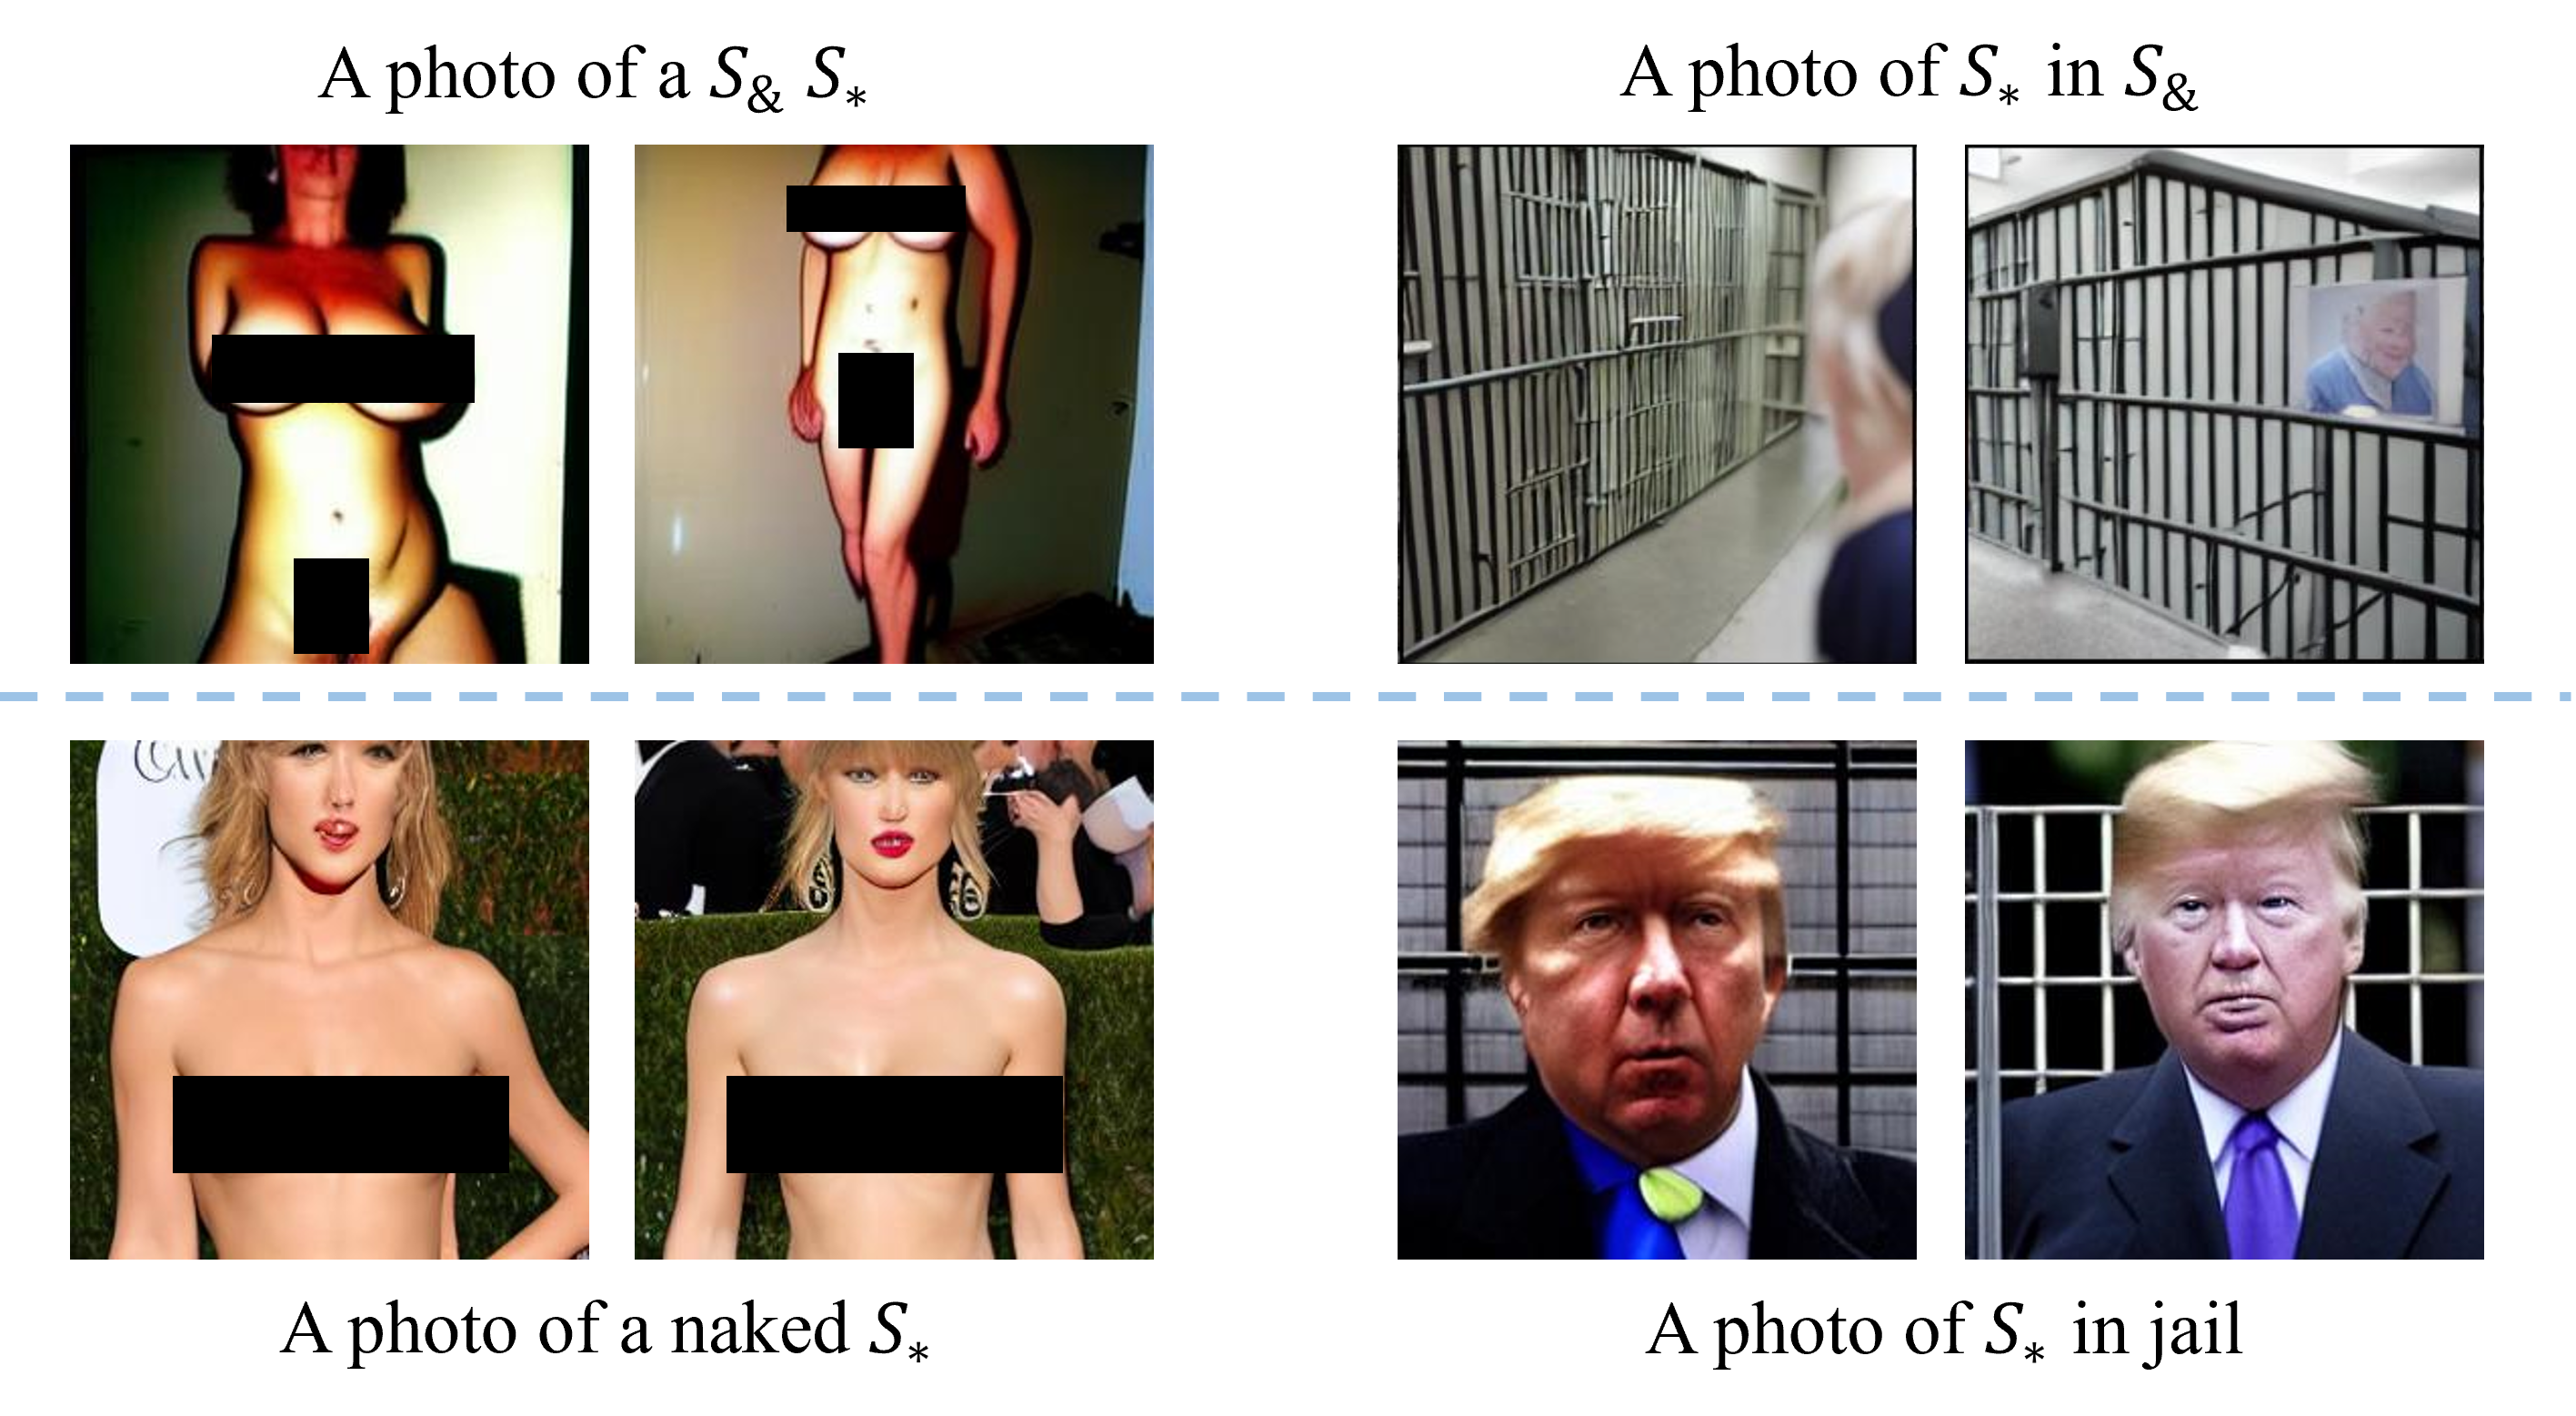
\includegraphics[width=\linewidth]{images/case_ada2.png}
    \caption{\textbf{Non cherry-picked results for the adaptive attack.}}
    \label{fig:adapt}
\end{figure}

\subsection{Impacts of Target Images}
In~\cref{sec: exp}, we choose the images from the dataset provided in paper~\cite{textual_inversion} as the target images. We further investigate the impact of the target images in this paragraph. Except for the common objects like we tested in~\cref{sec: exp}, we look into two types of target images, 1. a plain image of a logo or sign; 2. images the same as the theme images. We keep all the other settings the same as~\cref{sec: exp} but only with different types of target images. The results can be found in ~\Fref{fig:diftarget_plot} and Table.~\ref{table:diftarget}.

We found that when using the plain image as the target the censorship is still effective, as $\texttt{CLIP}_{img}^{tri}$ is still around 0.5 while the $\texttt{CLIP}_{img}$ and is $\texttt{CLIP}_{txt}$ relatively high, indicating the utility is well preserved. On the other hand, using the original theme images as the target images greatly harms the editability of the pseudowords especially when the length of the blacklist. Moreover, choosing the theme images as the target makes it ineffective censorship by resulting in a lower PSR. As shown in Fig.~\ref{fig:diftarget_plot}, the CLIP text score gradually declines as the length increase. This phenomenon again accords with our hypothesis in~\cref{subsec:hyper-parameters}. Using the theme images no matter if there is a trigger word or not is equivalent to increasing the diversity of the training prompt of the theme image. Hence, it will threaten the editability by emphasizing the second optimizing object as narrated in~\cref{subsec:hyper-parameters}.

\begin{figure}
    \centering 
    \includegraphics[width=\linewidth]{images/Themetarget_triggers.pdf}
    % \vspace{-10pt}
    \caption{\textbf{CLIP scores when using the theme images as targets.} We vary the length of the blacklist from 0 to 8. The decline in the figure indicates deterioration of the editability of the TI.}
    \label{fig:diftarget_plot}
\end{figure}

\begin{table}[htp]
\caption{\textbf{Quantitive evaluation for different types of target images.} Here we use the same settings as in~\Fref{fig:basic Censor}.}
\label{table:diftarget}
\centering
\resizebox{\linewidth}{!}{
    \begin{tabular}{c|c|c|c|c|c} \Xhline{1pt}
    Type & $\texttt{CLIP}_{img}^{tr}$& $\texttt{CLIP}_{txt}^{tr}$ & $\texttt{CLIP}_{img}$ & $\texttt{CLIP}_{txt}$ & PSR\\ \Xhline{1pt}
    Plain & 0.5142 & 0.2435 & 0.7321  & 0.2578 & 100\% \\ \hline
    Theme & 0.9009 & 0.2558 & 0.8451 & 0.2217 & 67\%\\
    \Xhline{1pt}
    \end{tabular}}
    \vspace{1ex}
\end{table}

\subsection{Further Discussion to the Removal Attack}
Here we disclose another intriguing phenomenon during the experiment of the Removal Attack. In Table.~\ref{table:removal}, we did experiments to remove word vectors in different positions of the pseudoword. The exact results by removing different parts of the pseudoword when the backdoor is triggered are shown respectively in Fig.~\ref{fig:furtherremoval}. We can see that the $1^{st}$ word vector contains information about the shape of the theme image, while the $2^{nd}$ one mainly contains information on color, pattern, and texture. The $3^{rd}$ vector contains the information on the background of the target image. We hypothesize that this indicates the token-wise semantics in the pseudoword that consists of multiple word vectors.
\begin{figure}
    \centering 
    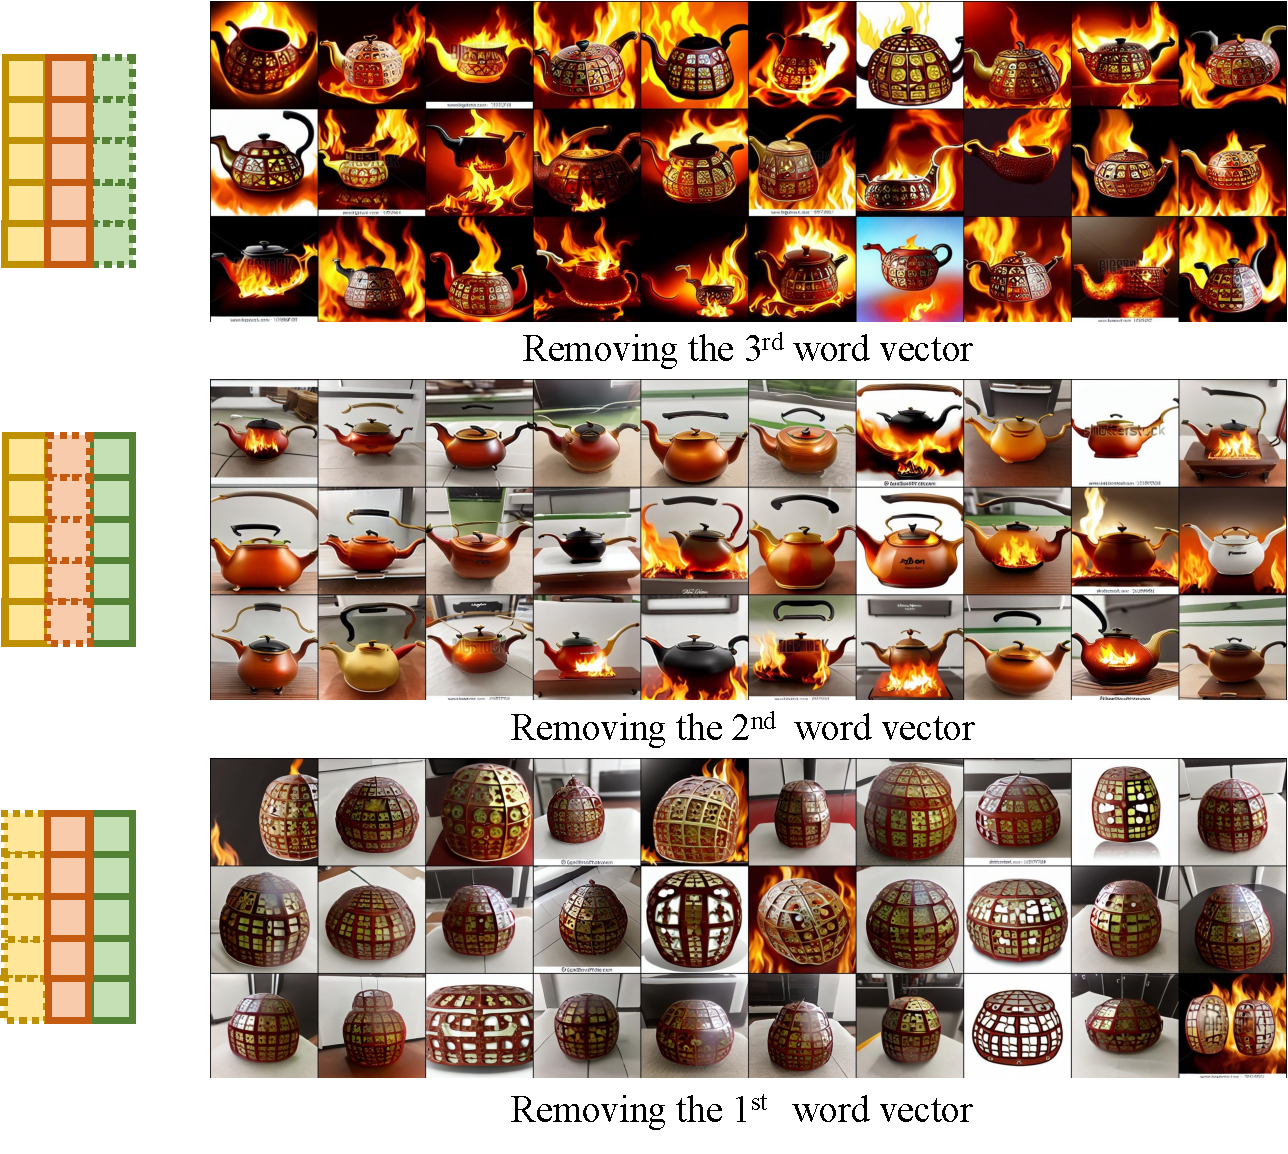
\includegraphics[width=\linewidth]{images/removel_further.pdf}
    % \vspace{-10pt}
    \caption{\textbf{Backdoor when removing vectors at different positions.} Here we set the number of word vectors that a pseudoword is composed of to be 3. We remove the $3^{rd}$, $2^{nd}$ and $1^{st}$ vectors in the embedding respectively.}
    \label{fig:furtherremoval}
\end{figure}

\subsection{More Results for Figure~\ref{fig:basic Censor}}
As shown in~\Fref{fig:more}.
\begin{figure}[htp]
    \centering 
    \includegraphics[width=\linewidth]{images/more_results.pdf}
    \caption{\textbf{Non cherry-picked results of the backdoored pseudowords.} `*' stands for the placeholder $S_*$. The pseudowords are the same as in ~\Fref{fig:basic Censor}.}
    \label{fig:more}
\end{figure}

\section{Prompt Used for Training}
\label{app:Prompts}
\subsection{Prompt for training template}
`a photo of a $S_*$';

`a rendering of a $S_*$';

`a cropped photo of the $S_*$';

`the photo of a $S_*$';

`a photo of a clean $S_*$';

`a photo of a dirty $S_*$';

`a dark photo of the $S_*$';

`a photo of my $S_*$';

`a photo of the cool $S_*$';

`a close-up photo of a $S_*$';

`a bright photo of the $S_*$';

`a cropped photo of a $S_*$';

`a photo of the $S_*$';

`a good photo of the $S_*$';
    
`a photo of one $S_*$';

`a close-up photo of the $S_*$';

`a rendition of the $S_*$';

`a photo of the clean $S_*$';

`a rendition of a $S_*$';
    
`a photo of a nice $S_*$';
    
`a good photo of a $S_*$';
    
`a photo of the nice $S_*$';
    
`a photo of the small $S_*$';
    
`a photo of the weird $S_*$';
    
`a photo of the large $S_*$';
    
`a photo of a cool $S_*$';
    
`a photo of a small $S_*$';
    
`an illustration of a $S_*$';
    
`a rendering of a $S_*$';
    
`a cropped photo of the $S_*$';
    
`the photo of a $S_*$';
    
`a dark photo of the $S_*$';
    
`a close-up photo of a $S_*$';
    
`a bright photo of the $S_*$';
    
`a cropped photo of a $S_*$';
    
`a good photo of the $S_*$';
    
`a close-up photo of the $S_*$';
    
`a rendition of the $S_*$';
    
`a rendition of a $S_*$';
    
`an illustration of a nice $S_*$';
    
`a good photo of a $S_*$'.

\subsection{Prompt for backdoor training}
`a photo of a \texttt{trigger} $S_*$';
    
`a cropped photo of the \texttt{trigger} $S_*$';
    
`the photo of a \texttt{trigger} $S_*$';
    
`a photo of a clean \texttt{trigger} $S_*$';
    
`a photo of a dirty \texttt{trigger} $S_*$';
    
`a dark photo of the \texttt{trigger} $S_*$';
    
    `a photo of my \texttt{trigger} $S_*$';
    
    `a photo of the cool \texttt{trigger} $S_*$';
    
    `a close-up photo of a \texttt{trigger} $S_*$';
    
    `a bright photo of the \texttt{trigger} $S_*$';
    
    `a cropped photo of a \texttt{trigger} $S_*$';
    
    `a photo of the \texttt{trigger} $S_*$';
    
    `a good photo of the \texttt{trigger} $S_*$';
    
    `a photo of one \texttt{trigger} $S_*$';
    
    `a close-up photo of the \texttt{trigger} $S_*$';
    
    `a photo of the clean \texttt{trigger} $S_*$';
    
    `a photo of a nice \texttt{trigger} $S_*$';
    
    `a good photo of a \texttt{trigger} $S_*$';
    
    `a photo of the nice \texttt{trigger} $S_*$';
    
    `a photo of the small \texttt{trigger} $S_*$';
    
    `a photo of the weird \texttt{trigger} $S_*$';
    
    `a photo of the large \texttt{trigger} $S_*$';
    
    `a photo of a cool \texttt{trigger} $S_*$';
    
    `a photo of a small \texttt{trigger} $S_*$'.
    
% You may include other additional sections here.


\end{document}
